\subsection{Ángulos de Euler}
% CAMBIAR EJES MINÚSCULAS A EJES PRIMADOS
% PONER PARA QUÉ ES EL ÁNGULO N. ESTABLECEN EL ANGULO DE ROTACIÓN.
% TROMPO DESCRIBIENDO LOS MOVIMIENTOS DE LAS ROTACIONES
%ANGULO DEL PLANO DE ROTACIÓN
%

Los ángulos de Euler constituyen un conjunto de tres coordenadas angulares que
sirven para especificar la orientación de un sistema de referencia de ejes
ortogonales, normalmente móvil, respecto a otro sistema de referencia de ejes
ortogonales normalmente fijos.

Dados dos sistemas de coordenadas $xyz$ y $XYZ$ con origen común, es posible
especificar la posición de un sistema en términos del otro usando tres ángulos
$\alpha$, $\beta$, $\gamma$.

La definición matemática es estática y se basa en escoger dos planos, uno en el
sistema de referencia y otro en el triedro rotado. En el esquema adjunto serían
los planos $xy$ y $XY$. Escogiendo otros planos se obtendrían distintas convenciones
alternativas, las cuales se llaman de Tait-Bryan cuando los planos de referencia
son no-homogéneos (por ejemplo $xy$ y $XY$ son homogéneos, mientras $xy$ y $XZ$ no lo
son).

La intersección de los planos coordenados $xy$ y $XY$ escogidos se llama línea de
nodos, y se usa para definir los tres ángulos:

\begin{itemize}
    \item $\alpha$ es el ángulo entre el eje x y la línea de nodos.
    \item $\beta$  es el ángulo entre el eje z y el eje Z.
    \item $\gamma$  es el ángulo entre la línea de nodos y el eje X.
\end{itemize}

más adelante se establecerá que los tres ángulos de Euler descritos son los
valores de las tres rotaciones intrínsecas que describen el sistema.

Notar que también se considera la notación: $\alpha =\phi$, $\gamma =\psi$,
$\beta =\theta$

Las rotaciones de Euler son los movimientos resultantes de variar uno de los
ángulos de Euler dejando fijo los otros dos. Son los siguientes:

\begin{itemize}
    \item Preseción
    \item Nutación
    \item Rotación intrínseca
\end{itemize}

Si escribimos la rotación de ángulos $\phi$
,$\theta$ ,$\psi$ como una composición de estas tres rotaciones:

\begin{equation}
    A(\phi ,\theta ,\psi )=R(\phi ,\theta ,\psi )N(\phi ,\theta )P(\phi)\
\end{equation}

entonces se cumple:

\begin{equation}
    \begin{array}{ll}
    A(\delta \phi +\phi ,\theta ,\psi ) & = P(\delta \phi )A(\phi ,\theta ,\psi) \\
    A(\phi ,\delta \theta +\theta ,\psi ) & = N(\phi ,\delta \theta )A(\phi ,\theta ,\psi ) \\
    A(\phi,\theta ,\delta \psi +\psi ) &=R(\phi ,\theta ,\delta \psi )A(\phi ,\theta ,\psi) \\
    \end{array}
\end{equation}

Como consecuencia de estas propiedades, estas rotaciones son conmutativas
entre ellas:

\begin{equation}
    P(\delta \phi )N(\delta \theta )A(\phi ,\theta ,\psi)=A(\delta \phi +\phi ,\delta \theta +\theta ,\psi )=N(\delta \theta )P(\delta \phi )A(\phi ,\theta ,\psi )
\end{equation}

lo que también podría verse intuitivamente usando la analogía entre los ángulos
de Euler y los de un soporte Cardán.

\begin{figure}[h]
    \centering
    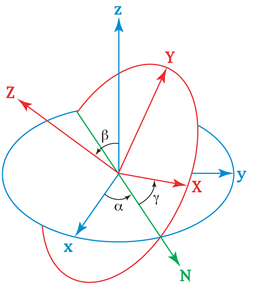
\includegraphics[scale=1]{figures/euler_angles.png}
    \caption{Dos sistemas de coordenadas ortogonales en el que se muestran los ángulos de Euler.}
    \label{fig:eulerAngles}
\end{figure}
